\chapter{Pruebas de integración y fiabilidad}

El eje fundamental de este capítulo es mostrar el rendimiento del algoritmo y la integración final en diferentes circunstancias, y probar que el mismo es capaz de desenvolverse de forma satisfactoria en la mayoría de escenarios posibles.

\section{Pruebas sobre el algoritmo de OCR}
Para corroborar el funcionamiento del algoritmo se ensayaron diversas pruebas, con la finalidad de testear el comportamiento del algoritmo sobre diferentes entornos de trabajo, partiendo desde un ambiente ideal para llegar a uno alejado de él en el cual no se puede garantizar el correcto funcionamiento.

\subsection{Pruebas de distancia y ángulo}
Para realizar esta serie de pruebas se colocó un Volkswagen Up modelo 2015 con patente PEY232 en una posición fija y se procedió a medir con una cinta métrica de error 1 cm. Para las mediciones se consideró que la cámara y la patente están paralelas y enfrentadas. Este escenario define el ángulo de $0^\circ$ y cambia solamente cuando la cámara gira en dirección paralela al suelo, mientras que el origen se tomó desde el centro de la misma.
En Fig. \ref{fig:sistema-medicion-angulos} se puede apreciar un esquema del sistema de ejes. La medición consistió en la captura de una fotografía con la cámara de los sistemas SL a una distancia y ángulo determinados. Luego, cada medición se procesó con el algoritmo de OCR.
Debido al espacio con el que se contaba, se realizaron dos pruebas: la primera consistió en fijar el angulo en $0^\circ$ e ir tomando muestras cada 50cm, mientras que en la segunda se fijó la distancia en 50 cm y se vario el ángulo cada $30^\circ$.
Las muestras obtenidas para la primera prueba pueden verse en la Fig. \ref{fig:fotos-distancia} y los resultados obtenidos en la Tab. \ref{tab:resumen-distancia}, mientras que para la segunda prueba las muestras se observan en la Fig. \ref{fig:fotos-angulo} y los resultados en la Tab. \ref{tab:resumen-angulo}.


\begin{figure}[bth]
    \centering
    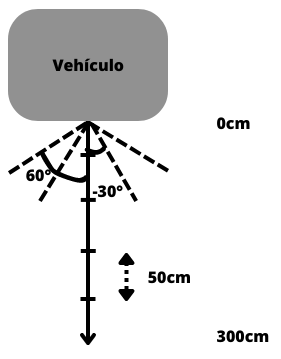
\includegraphics[width=.3\textwidth]{imgs/sistema-referencia.png}
    \caption{Sistema de referencia.}
    \label{fig:sistema-medicion-angulos}
\end{figure}

\begin{table}
    \centering
    \begin{tabular}{rl}
    \toprule
    Distancia & Predicción \\
    \midrule
    50        & PEY232     \\
    100       & PEY232     \\
    150       & PEY232     \\
    200       & PEY232     \\
    250       & PEY232     \\
    300       & PEY232     \\
    \bottomrule
\end{tabular}

    \caption{Resumen de la prueba de distancia a $0^\circ$ grados.}
    \label{tab:resumen-distancia}
\end{table}

\begin{table}
    \centering
    \begin{tabular}{rl}
    \toprule
    Ángulo & Predicción \\
    \midrule
    -60    & PEY232     \\
    -30    & PEY232     \\
    0      & PEY232     \\
    30     & PEY232     \\
    60     & PEY232     \\
    \bottomrule
\end{tabular}

    \caption{Resumen de la prueba de ángulos a 50 cm.}
    \label{tab:resumen-angulo}
\end{table}

\begin{figure}[bth]
    \centering
    \begin{subfigure}{.3\textwidth}
        \centering
        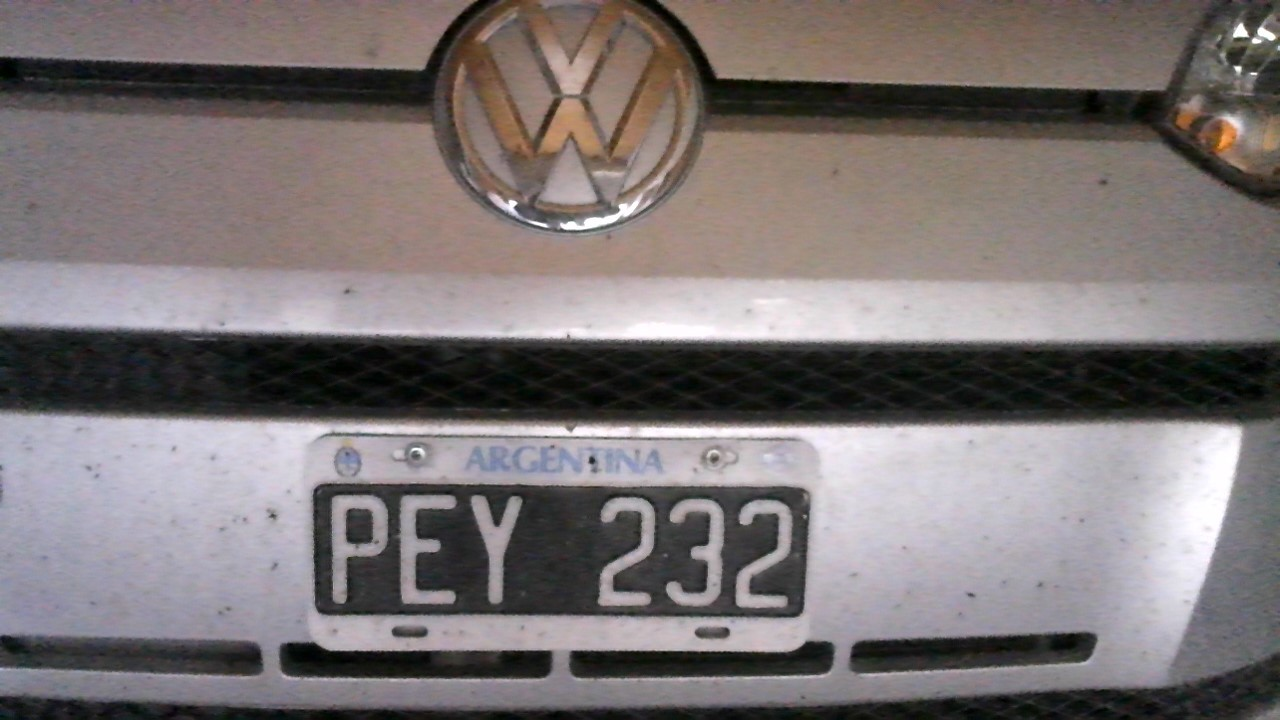
\includegraphics[width=\textwidth]{imgs/test-distancia/0_50.jpg}
        \caption{50cm}
    \end{subfigure}
    \begin{subfigure}{.3\textwidth}
        \centering
        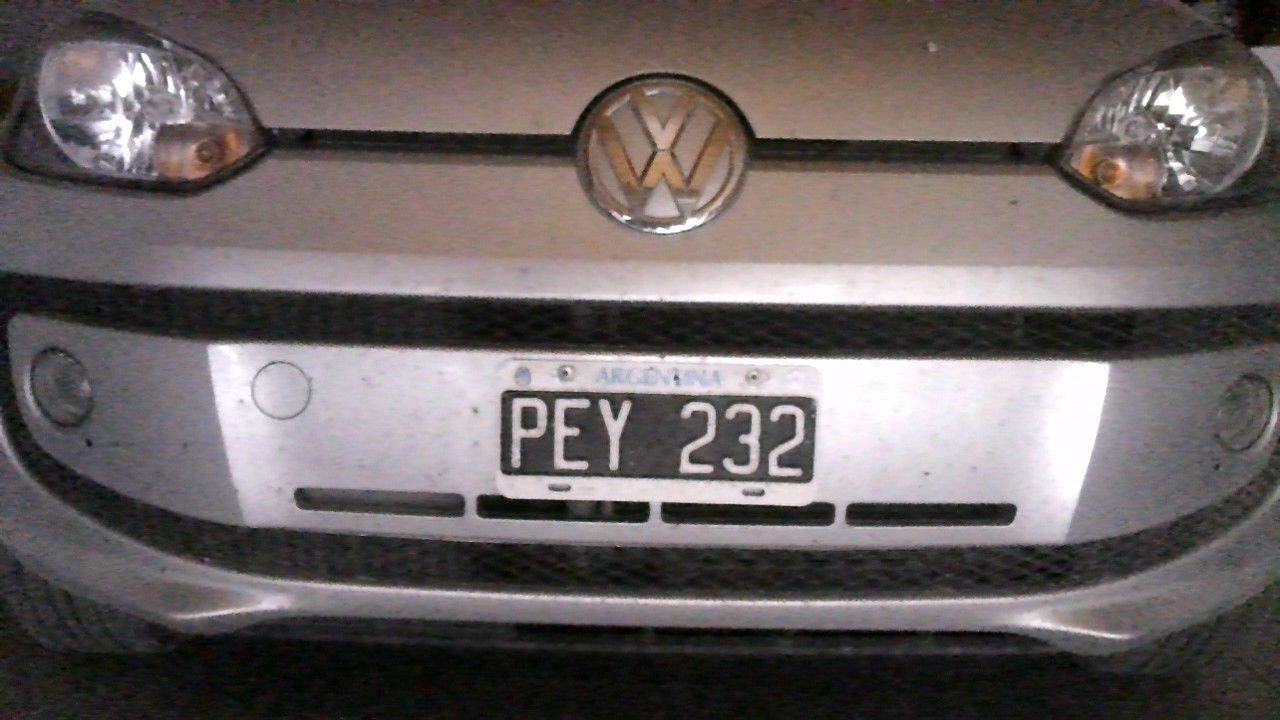
\includegraphics[width=\textwidth]{imgs/test-distancia/0_100.jpg}
        \caption{100cm}
    \end{subfigure}
    \begin{subfigure}{.3\textwidth}
        \centering
        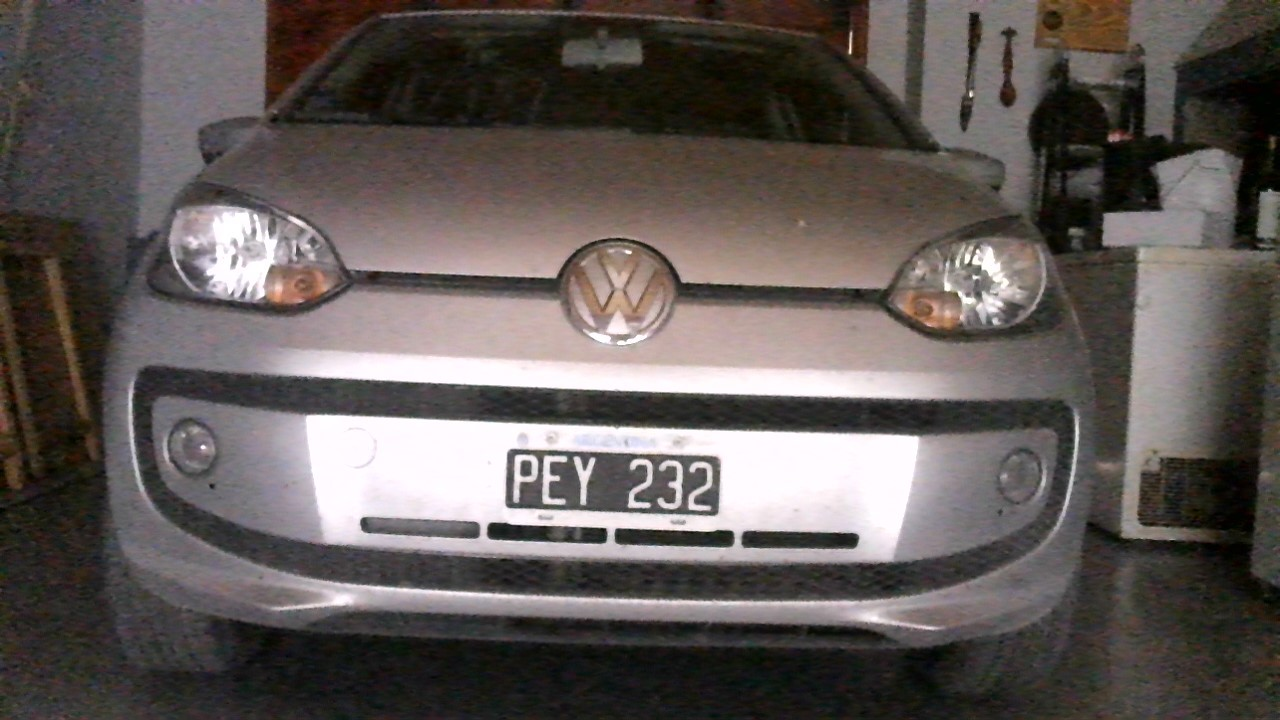
\includegraphics[width=\textwidth]{imgs/test-distancia/0_150.jpg}
        \caption{150cm}
    \end{subfigure}
    \begin{subfigure}{.3\textwidth}
        \centering
        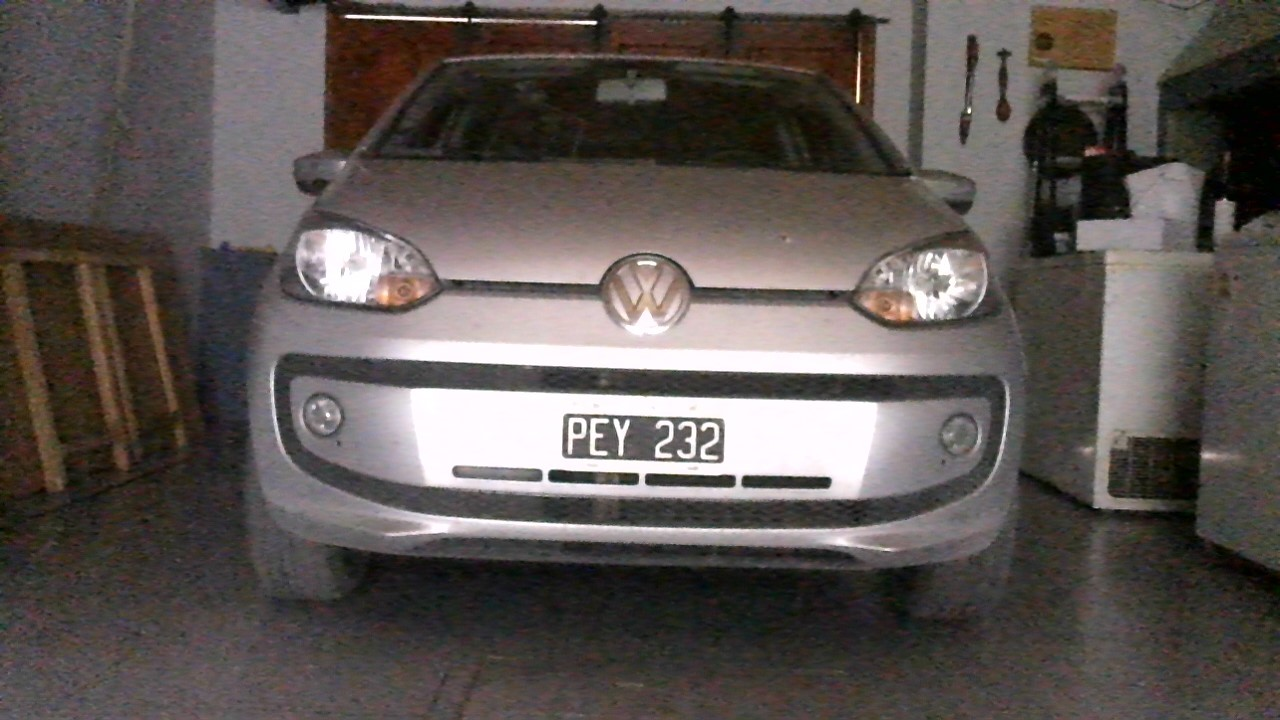
\includegraphics[width=\textwidth]{imgs/test-distancia/0_200.jpg}
        \caption{200cm}
    \end{subfigure}
    \begin{subfigure}{.3\textwidth}
        \centering
        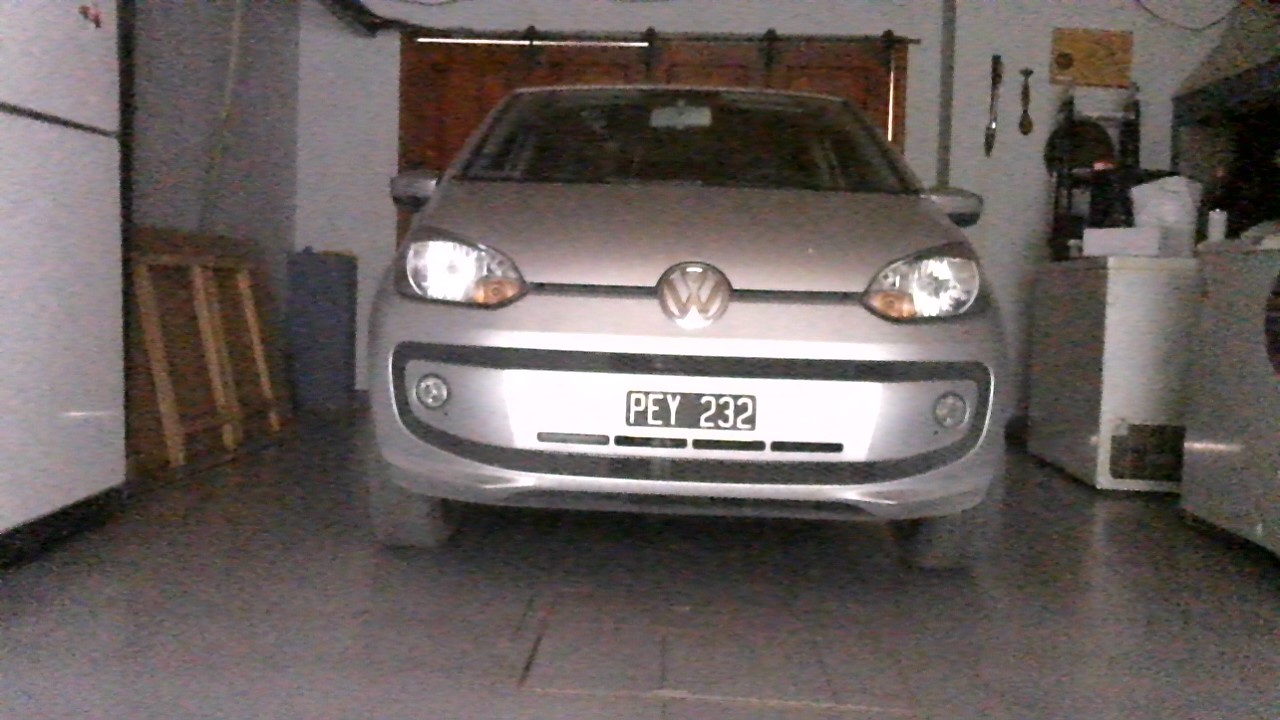
\includegraphics[width=\textwidth]{imgs/test-distancia/0_250.jpg}
        \caption{250cm}
    \end{subfigure}
    \begin{subfigure}{.3\textwidth}
        \centering
        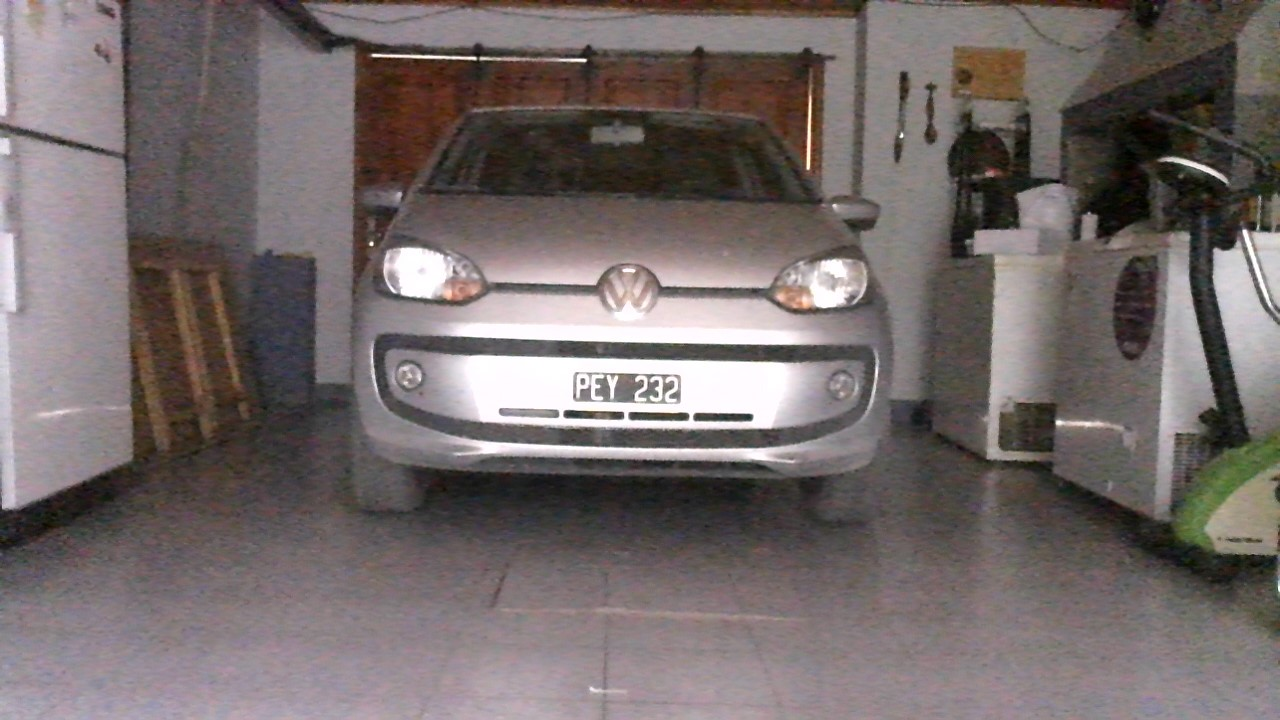
\includegraphics[width=\textwidth]{imgs/test-distancia/0_300.jpg}
        \caption{300cm}
    \end{subfigure}
    \caption{Fotografías a diferentes distancias.}
    \label{fig:fotos-distancia}
\end{figure}

\begin{figure}[bth]
    \centering
    \begin{subfigure}{.15\textwidth}
        \centering
        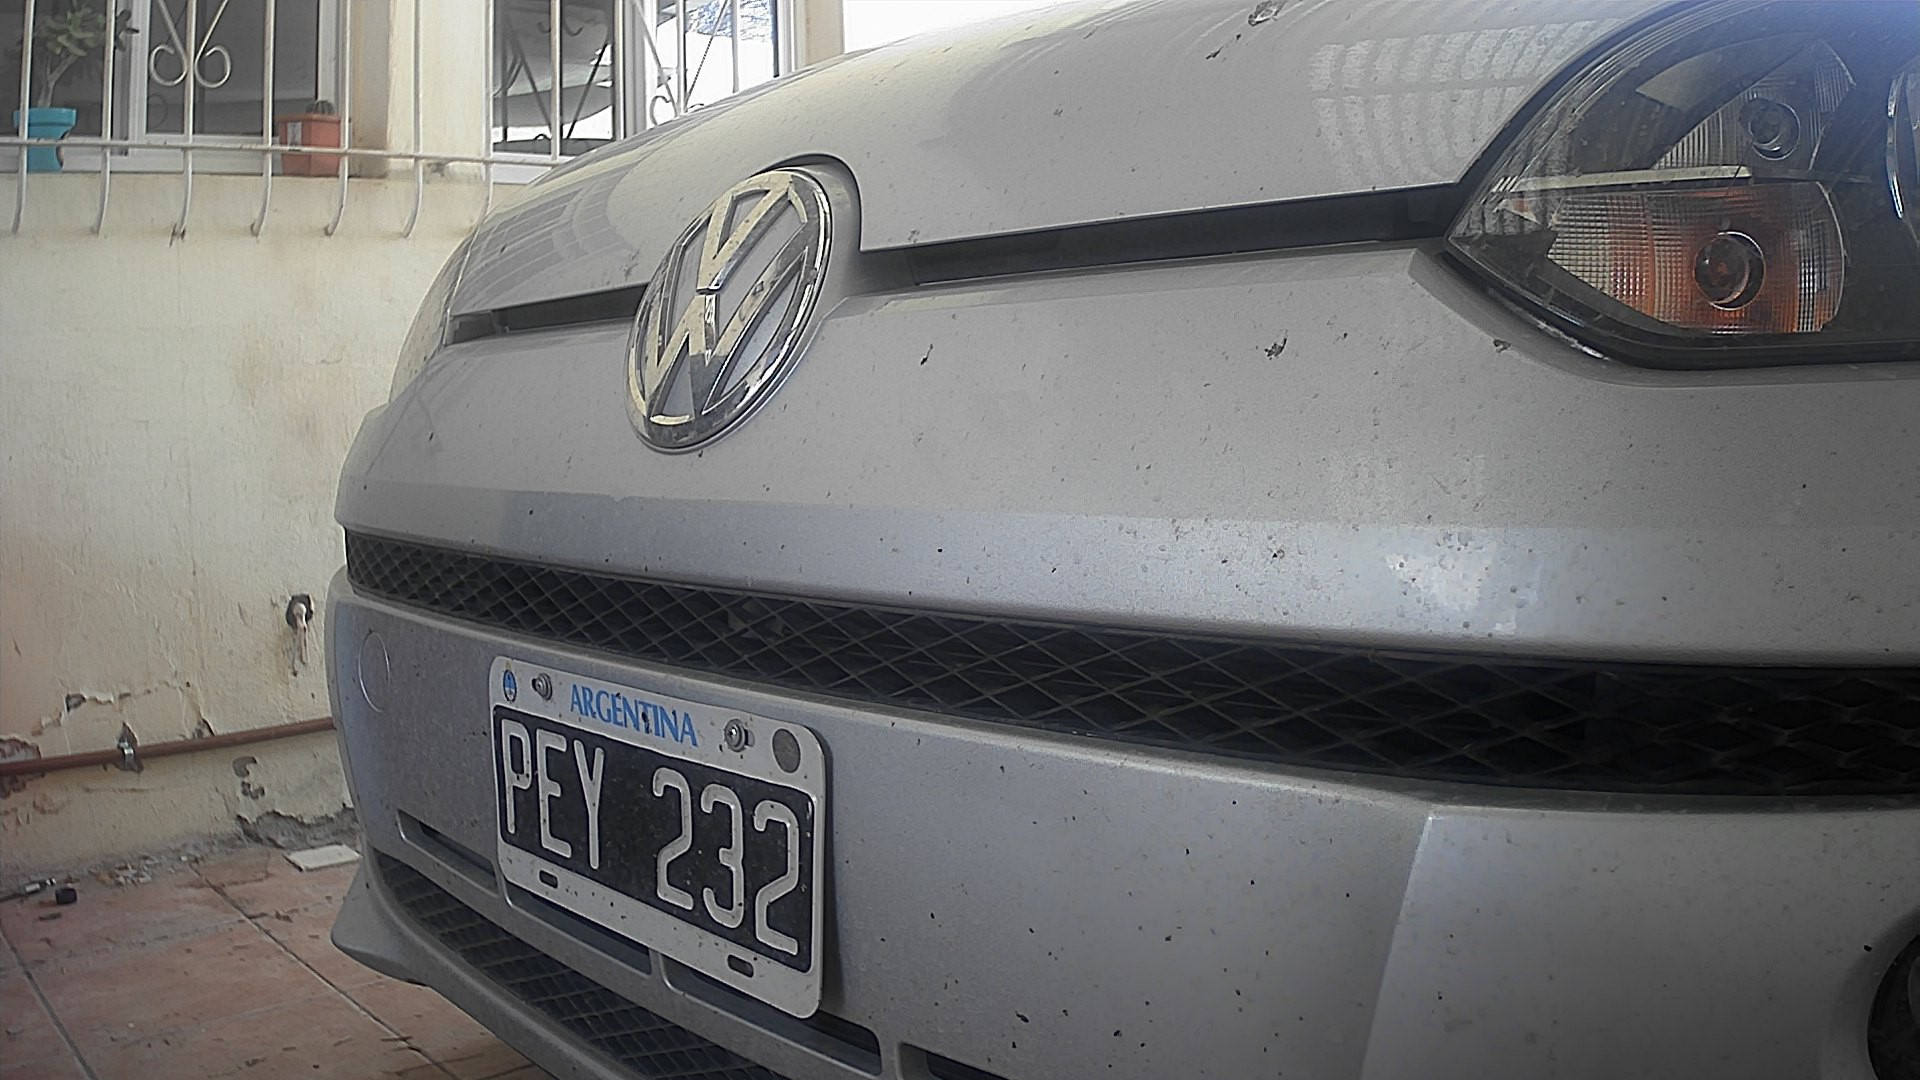
\includegraphics[width=\textwidth]{imgs/test-angulos/-60_50.jpg}
        \caption{$-60^\circ$}
    \end{subfigure}
    \begin{subfigure}{.15\textwidth}
        \centering
        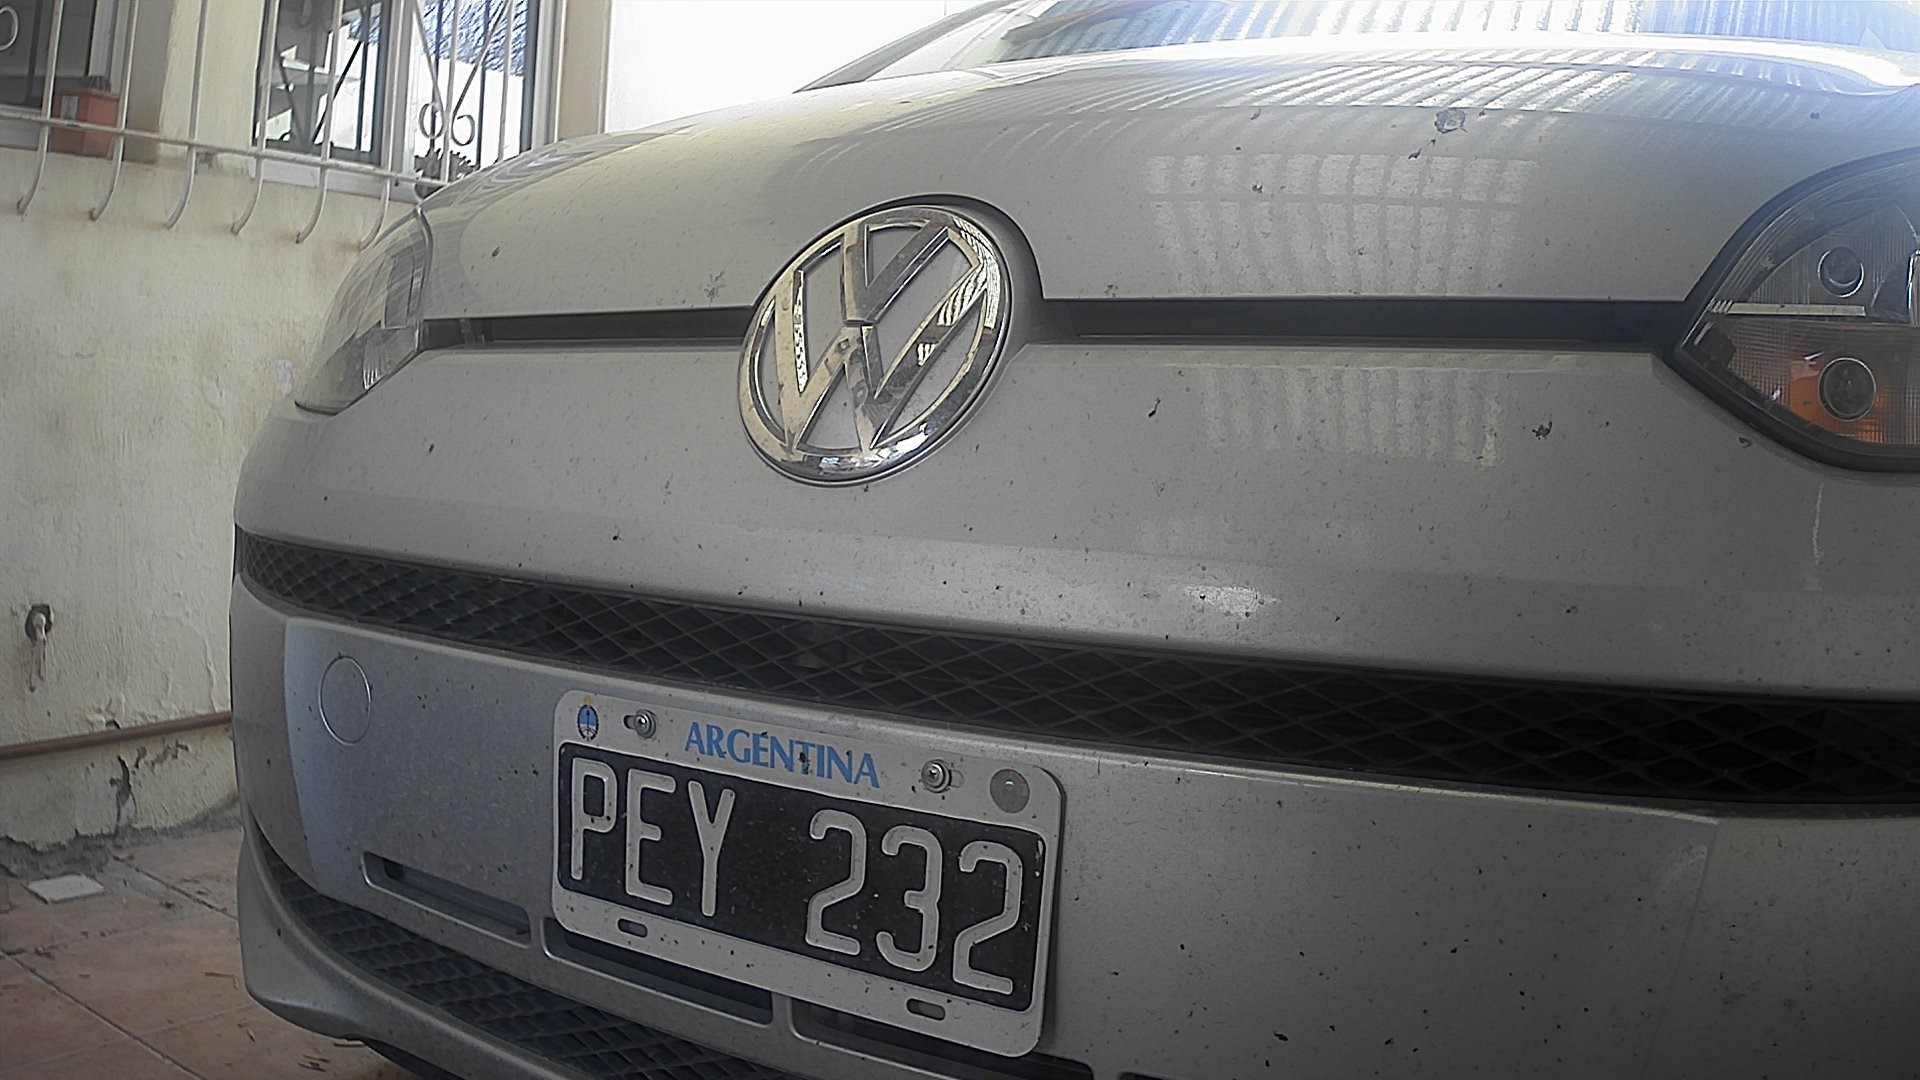
\includegraphics[width=\textwidth]{imgs/test-angulos/-30_50.jpg}
        \caption{$-30^\circ$}
    \end{subfigure}
    \begin{subfigure}{.15\textwidth}
        \centering
        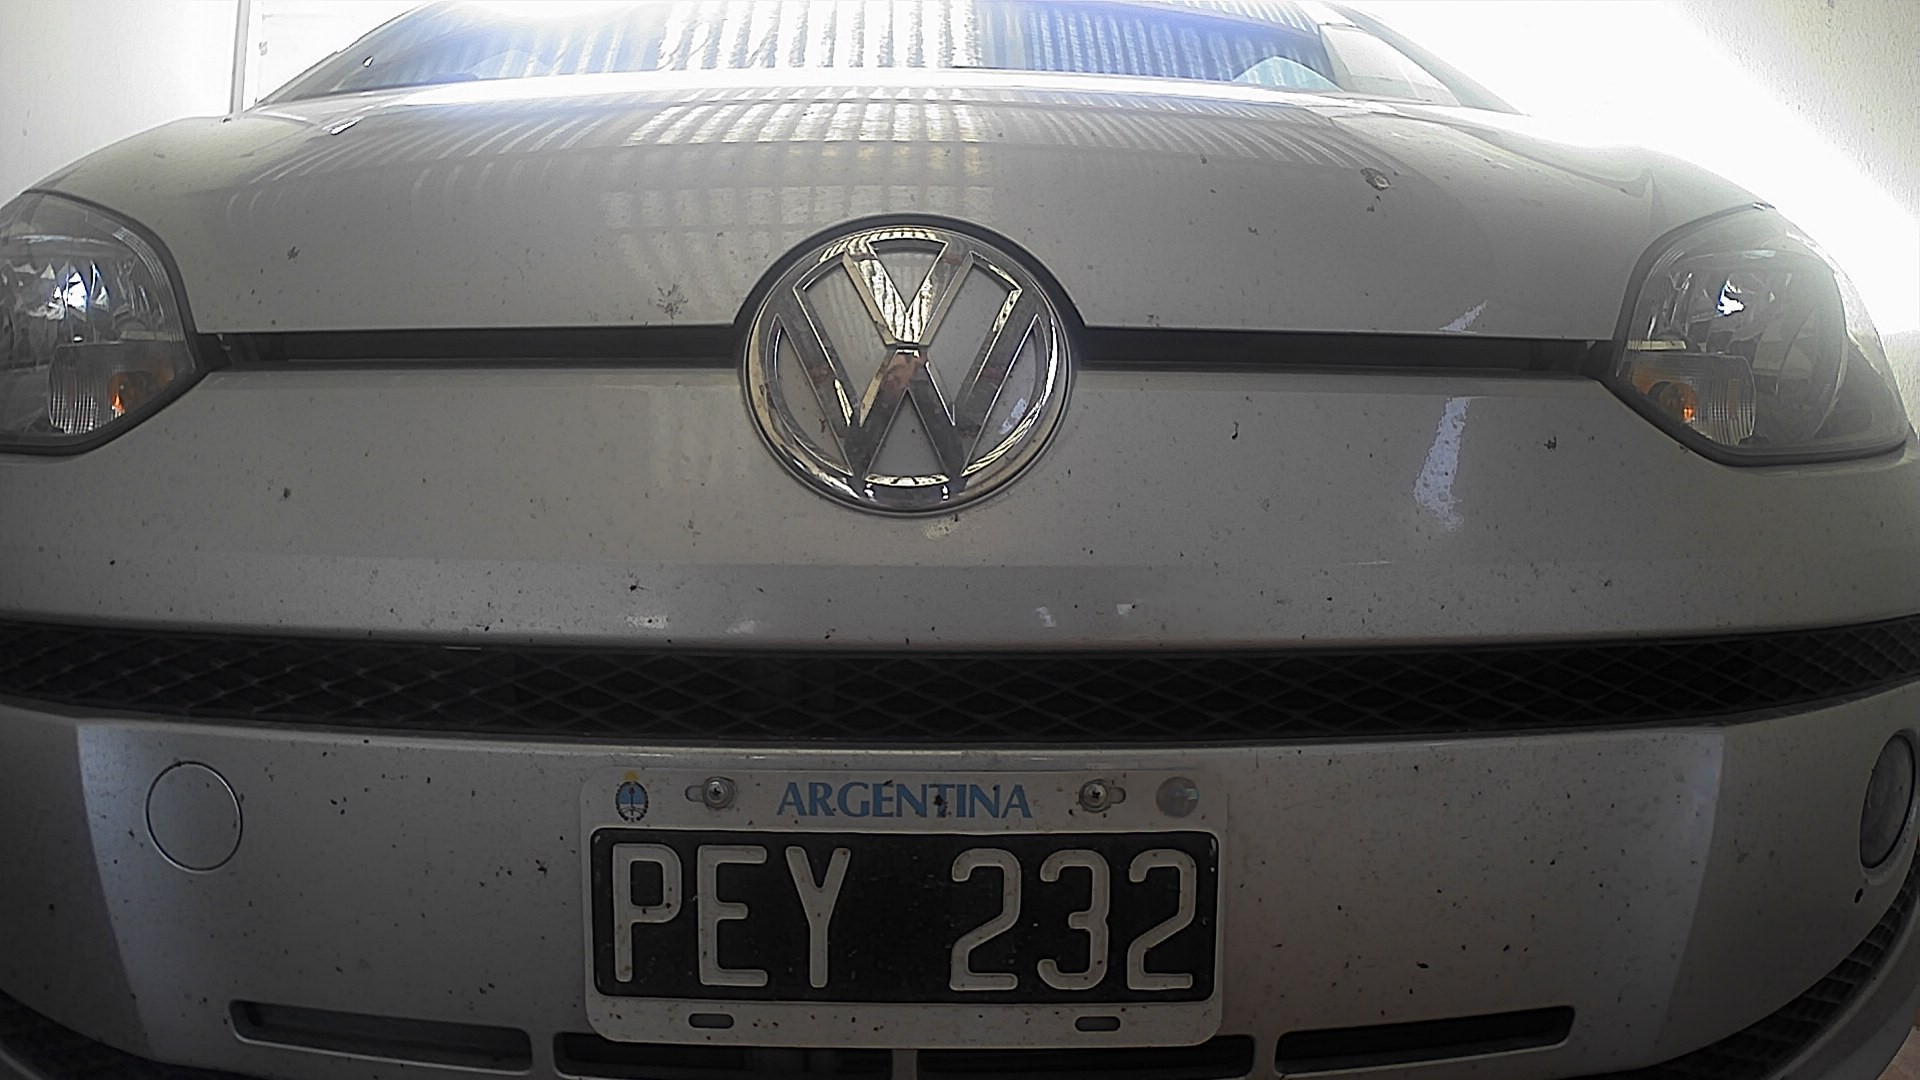
\includegraphics[width=\textwidth]{imgs/test-angulos/0_50.jpg}
        \caption{$0^\circ$}
    \end{subfigure}
    \begin{subfigure}{.15\textwidth}
        \centering
        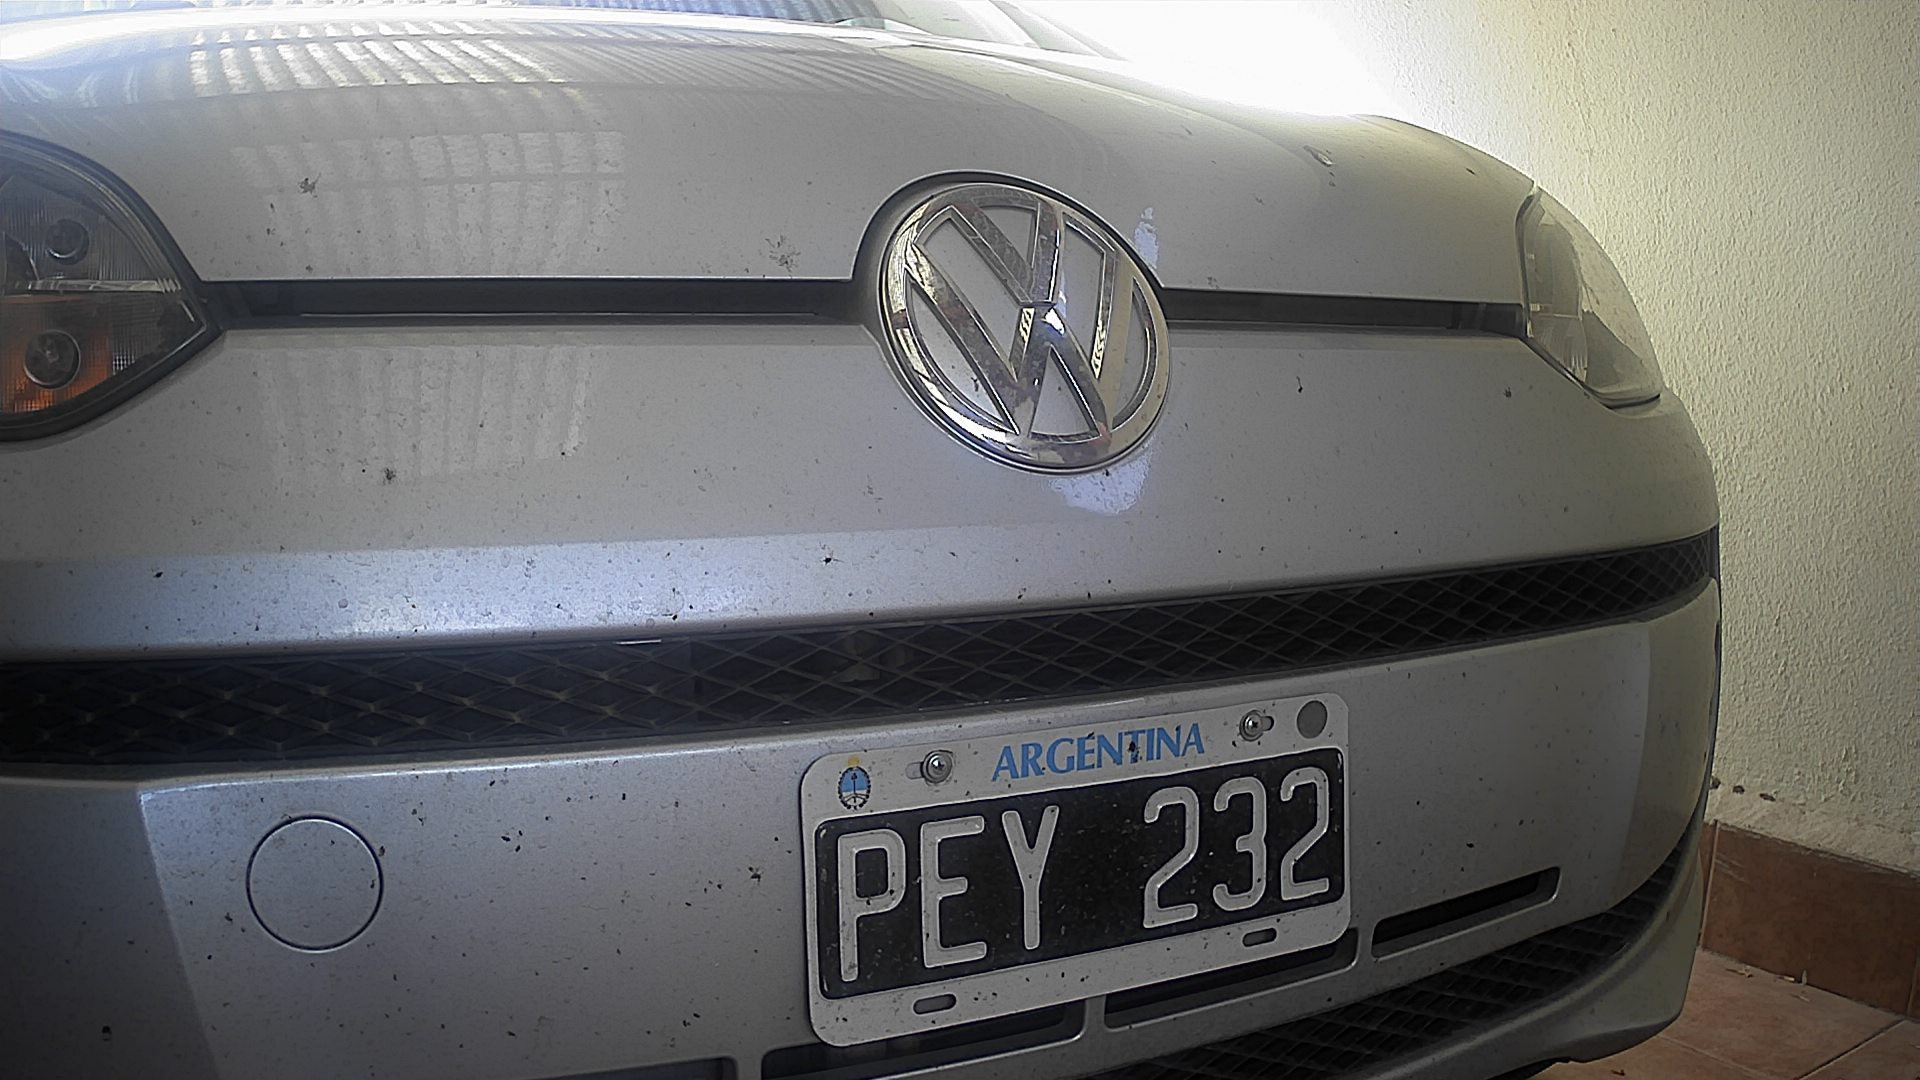
\includegraphics[width=\textwidth]{imgs/test-angulos/30_50.jpg}
        \caption{$30^\circ$}
    \end{subfigure}
    \begin{subfigure}{.15\textwidth}
        \centering
        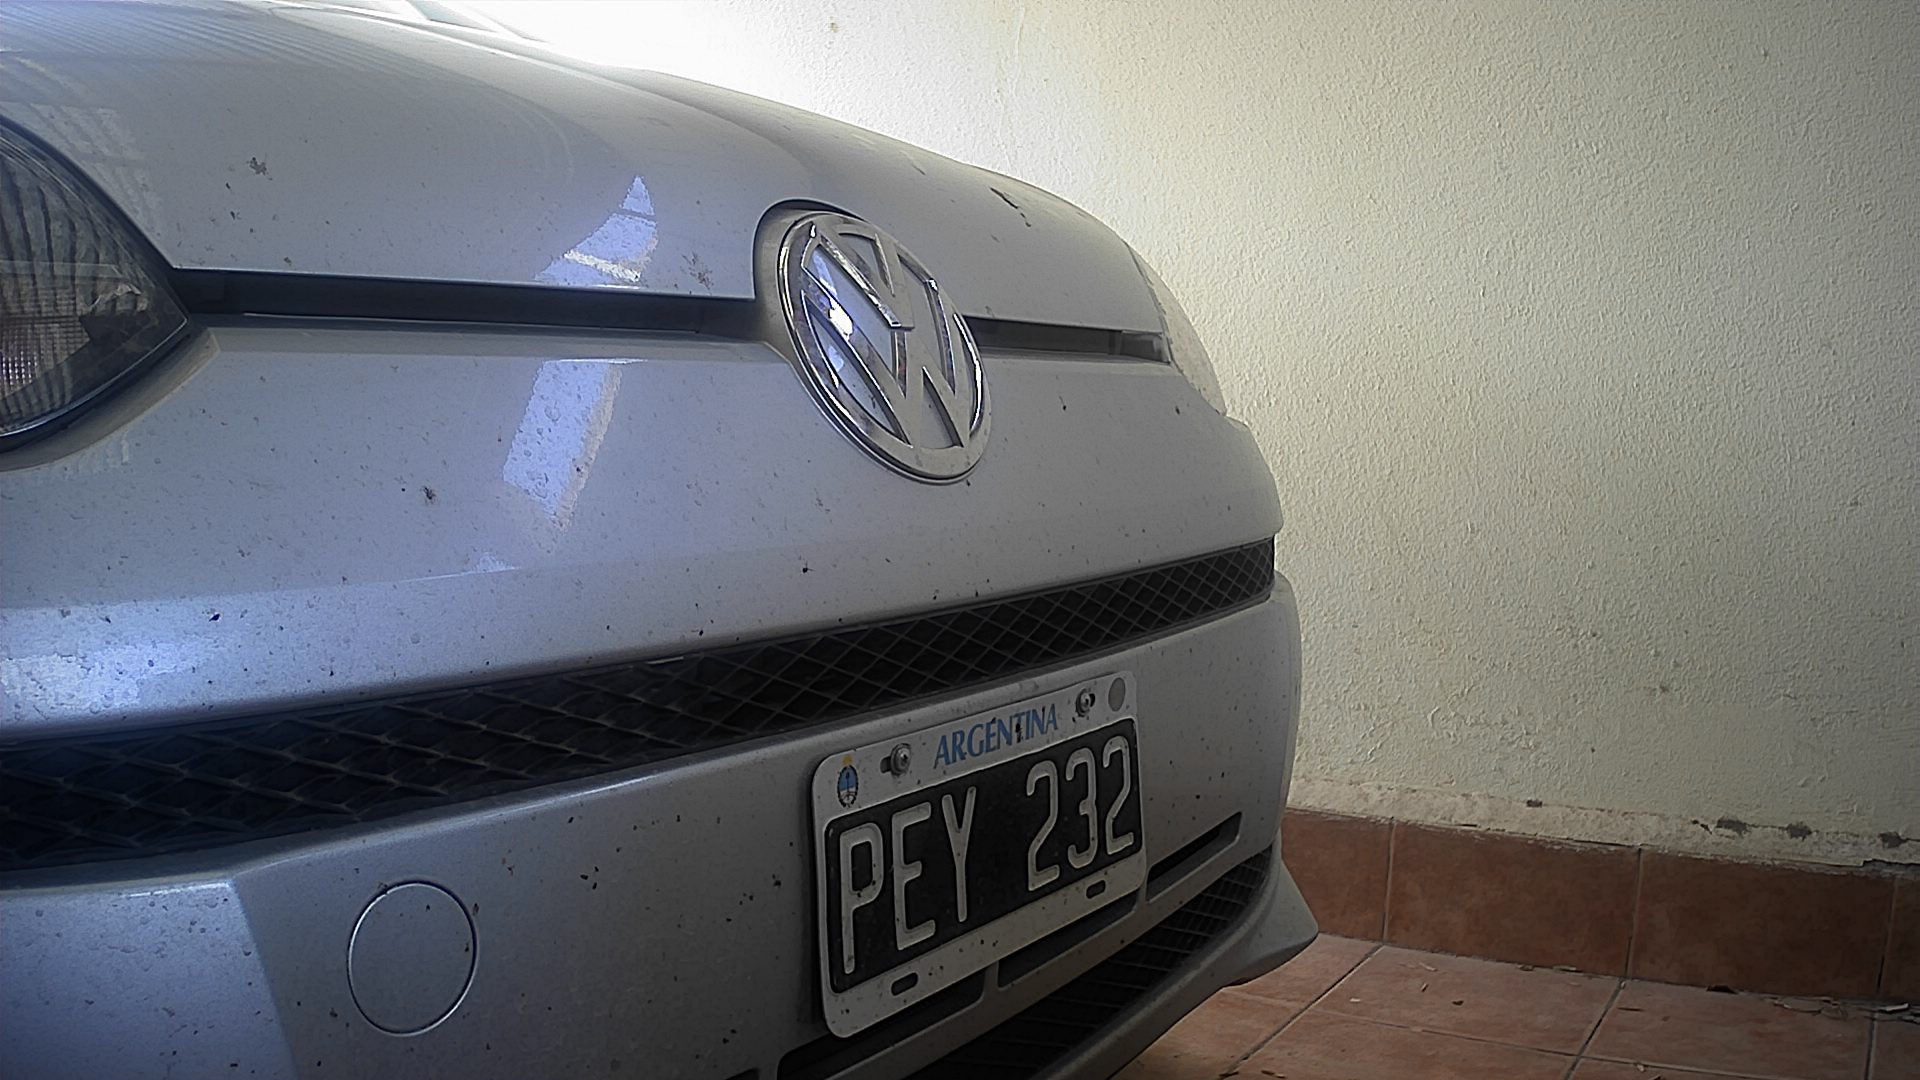
\includegraphics[width=\textwidth]{imgs/test-angulos/60_50.jpg}
        \caption{$60^\circ$}
    \end{subfigure}
    \caption{Fotografías a diferentes ángulos.}
    \label{fig:fotos-angulo}
\end{figure}

\subsection{Pruebas de exterior}
Esta prueba se realizó con una cámara Kanon PowerShot SX150 IS \cite{kanon_powershot_nodate} en el ingreso al estacionamiento de la Facultad de Ingeniería de la Universidad Nacional del Comahue entre las 8 y 9 de la mañana, el martes 6 de junio del 2023. La prueba se realizó colocando la cámara en un trípode con una altura de 70cm respecto del suelo\footnote{Se consideran los 60cm del tripode y los 10cm de la calzada, debido a que no era conveniente colocar la cámara sobre la calle.}, y se procedió a filmar los vehículos que entraban al estacionamiento o circulaban por la calle interna Libres Pensadores de la universidad. De este proceso de medición se obtuvieron dos videos de una duración aproximada de 40min.

Teniendo en cuenta que el algoritmo de OCR tarda 1200ms en procesar un frame es necesario realizar un filtrado, ya que los 40min de filmación equivalen en 72000 imágenes, y la mayoría no poseen vehículos o la patente no está enfocada.
El proceso de filtrado consistió en un recorte manual de las partes del video donde no había ningún vehículo, lo que terminó dejando 7min de filmación. Si bien este número es bajo, llevó a obtener un total de 35 vehículos diferentes en distintos frames, suficientes para el análisis. Posteriormente se convirtió el video en frames, utilizando Open CV, para luego procesar las 11000 fotografías y eliminar en las que no era posible detectar la forma de una patente por un ser humano. Luego se obtuvieron 3600 fotografías, que se procesaron por el algoritmo de OCR y se descartaron todas las imágenes con porcentaje de seguridad inferior al $50\%$, la seguridad se define como el promedio de las probabilidades estimadas para cada carácter.

Las imágenes se clasificaron en una carpeta con el valor predicho por el algoritmo.
Finalmente se contabilizaron los errores generando el resumen de Tab. \ref{tab:resumen-patente}.

\begin{table}
    \centering
    \begin{tabular}{cccccccc}
    \toprule
    Caracteres & Perfectas & 1 error & 2 errores & 3 errores & 4 errores & 5 errores & $\sum$ \\
    \midrule
    6          & 60        & 78      & 25        & 10        & 3         & 0         & 176    \\
    7          & 282       & 185     & 49        & 5         & 1         & 1         & 523    \\
    $\sum$     & 342       & 263     & 74        & 15        & 4         & 1         & 699    \\
    \bottomrule
\end{tabular}

    \caption{Resumen de las patentes reconocidas.}
    \label{tab:resumen-patente}
\end{table}


\subsection{Análisis de resultados}

En base a las pruebas de interior, se logra apreciar que el rendimiento del algoritmo de OCR en entonces controlados, vehiculo detenido, corta distancia y un angulo entre $-60^\circ$ y $60^\circ$, se obtienen resultados satisfactorios. Por otro lado, en la prueba de exterior, al contar con una diversidad de circunstancias tales como velocidad no nula, distancia y angulos fuera de los pensados, los resultados obtenidos cuentan con una baja eficiencia.


Realizando una analisis mas exaustivo de la prueba de exterior es posible obtener que la eficiencia del sistema ronda el $49\%$.
En la Tab. \ref{tab:resumen-patente} se observa que para patentes de seis caracteres la eficiencia ronda el $34\%$ esto se puede deber a que el dataset de entrenamiento contaba con una mayor tasa de patentes de siete caracteres o a que el estado de las patentes de seis caracteres al ser de mayor antigüedad se encuentran en peores condiciones lo que dificulta su estimación.
Por otro lado cuando se trata de patentes de siete caracteres estas poseen una eficiencia cercana al $54\%$, valor que se considera aceptable para esta prueba.
Se observa que para ambos casos la mayor tasa de error se da cuando existe un único carácter erróneo independientemente de su posición, por lo que en condiciones de obtención de la imagen más cercanas al de la primera prueba, aun cuando los vehículos tengan movimiento el porcentaje de acierto aumentaría considerablemente.

En base a estas pruebas se define que los limites para las condiciones de trabajo son:
\begin{enumerate}
    \item Distancia entre 50cm y 2m.
    \item Ángulo entre $-60^\circ$ y $60^\circ$.
    \item Velocidad de circulación paso de hombre.
\end{enumerate}
Los valores de distancia se toman teniendo en cuenta que el largo de un auto ronda los 4m \cite{duran_que_2023}, es por ello que se considera una distancia máxima de detección de 2m.
\section{Pruebas sobre el servidor}

\subsection{Integración de los sistemas SL y servidor}

Se montó un sistema SL mini junto con una notebook como servidor, el sistema montado se observa en la Fig. \ref{fig:pruebas-integracion-sl-server}, y se crearon registros de entrada, y cambio la configuración de un sistema SL en tiempo real. Con esta prueba se logró probar los cambios de configuración en tiempo real y que los registros se creen de forma correcta.

\begin{figure}
    \centering
    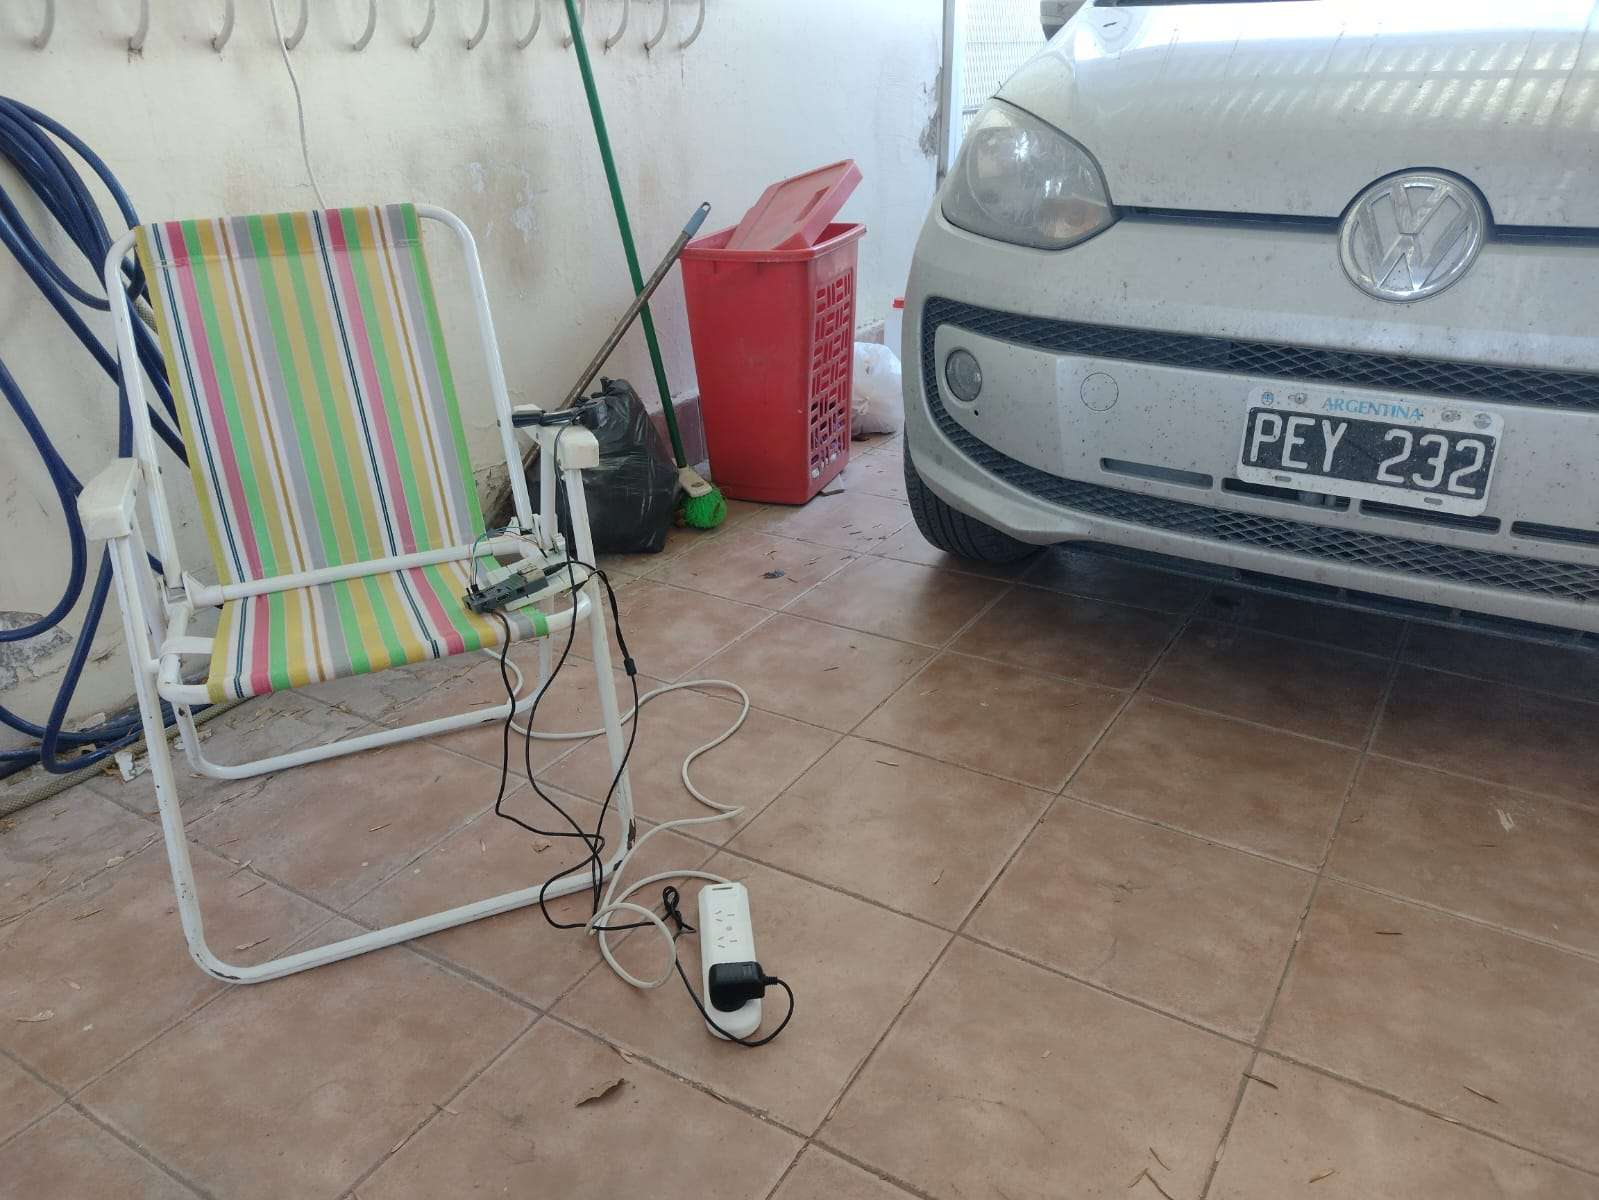
\includegraphics[width=.5\textwidth]{imgs/pruebas-server-garage.jpg}
    \caption{Sistema SL mini y servidor montados para lo pruebas de intregración.}
    \label{fig:pruebas-integracion-sl-server}
\end{figure}


\subsection{Creación de registros}

Para probar el correcto de funcionamiento del servidor, se creó un usuario de admin y un cliente. Se crearon dos lugares junto con un script en Python 3 emulando el envío de datos de las barreras, generando en el servidor 5900 registros para los lugares, probando el funcionamiento del sistema de inicio a fin los resultados de estas pruebas pueden observarse Fig. \ref{fig:dashboard}, algunos de los registros creados pueden apreciarse en la Fig. \ref{fig:registers}.

\section{Estado del prototipo}

En la actualidad se cuentan con 2 prototipos funcionales, uno para la versión SL y otro para el modelo SL mini.
El prototipo SL se encuentra montado sobre la placa Nvidia Jetson TX1 en su kit de desarrollo, la cual es capaz de correr el algoritmo de forma local.
Mientras que la versión SL mini se ejecuta en la placa Raspberry Pi 3 b+, que como se hizo mención en anterior capítulos no es capaz de correr el algoritmo de OCR por lo que esta tarea, se ejecuta en el servidor de prueba. El mismo se encuentra alojado en una notebook de la marca CX, la cual cuenta con un procesador Intel i5-1135G7, con 32 GB de ram, sin gpu dedicada, con lo que el tiempo de procesamiento por imagen es de 1,2s, como se mencionó en la Tab. \ref{tab:ocr}.
Para ambos modelos se cuenta con la misma cámara usb genérica y el sensor de distancia ultrasónico US-100.
Ambos prototipos se pueden apreciar en la Fig. \ref{fig:prototipos}.
\begin{figure}[bth]
    \begin{subfigure}{.45\textwidth}
        \centering
        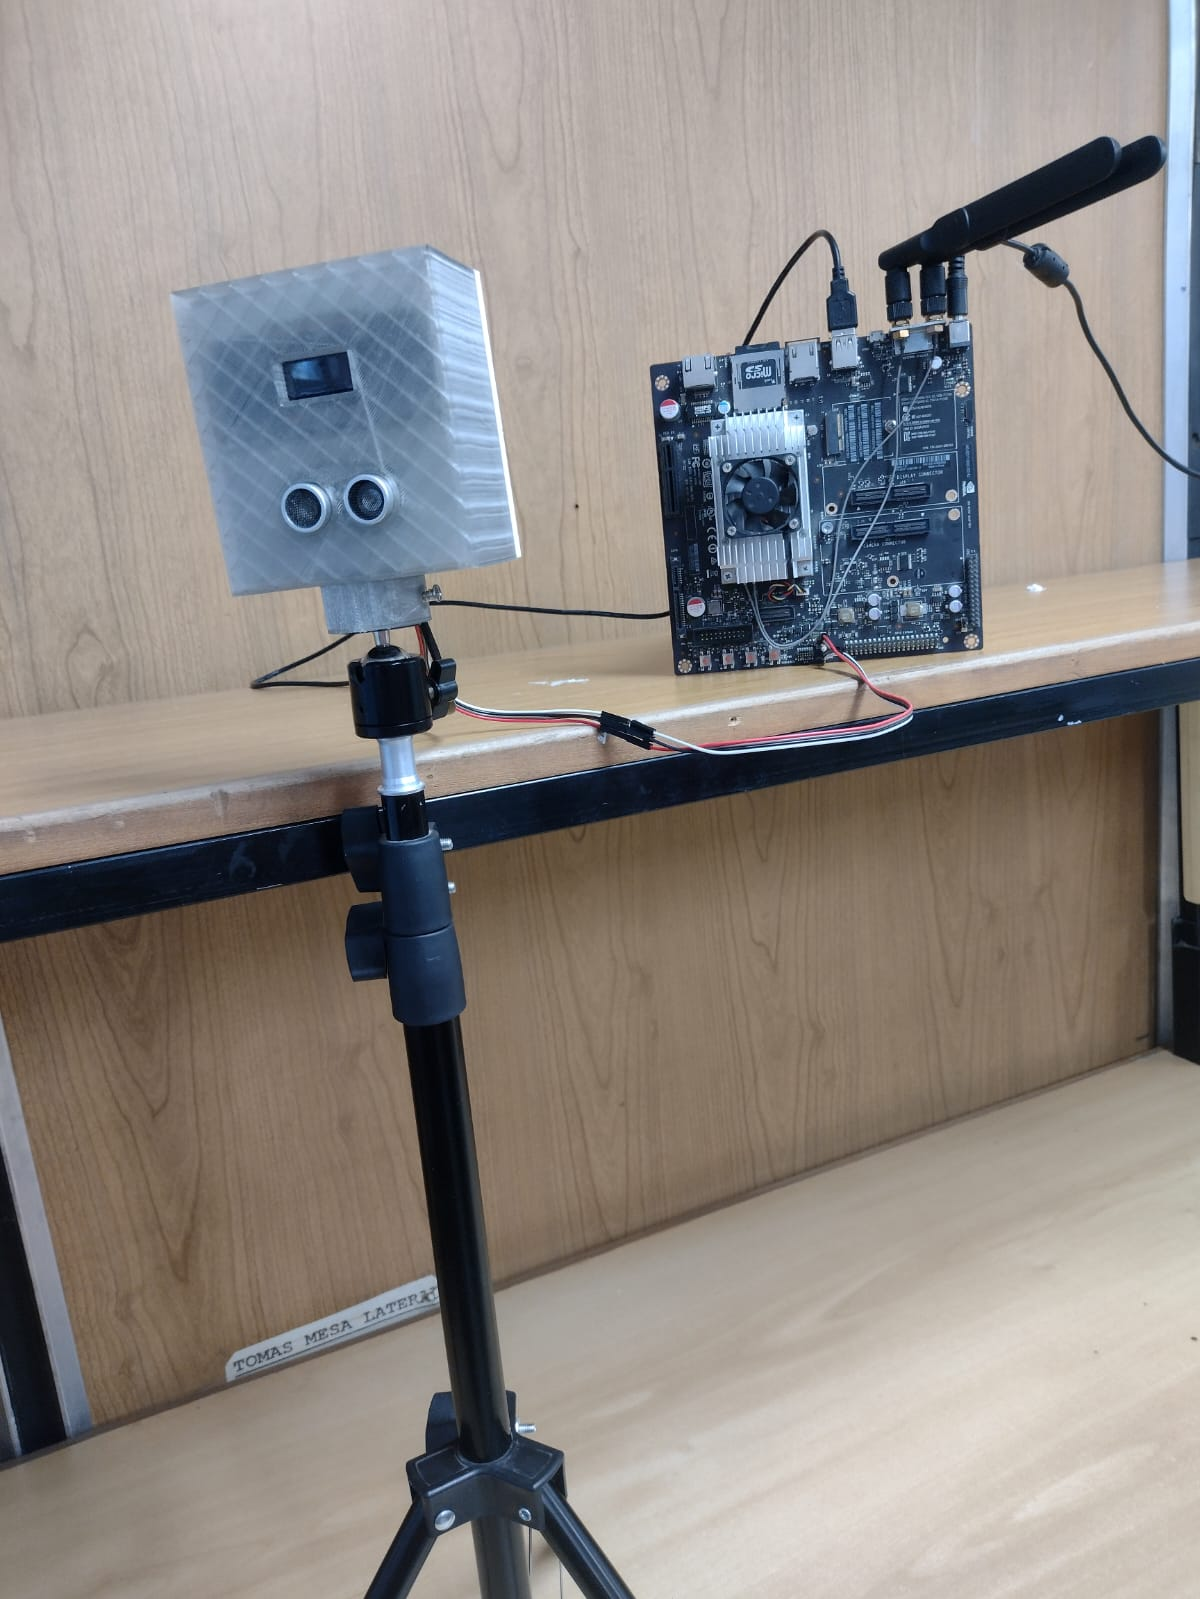
\includegraphics[height=5cm]{imgs/prototipo-sl.jpeg}
        \caption{Protipo SL.}
        \label{fig:prot-sl}
    \end{subfigure}
    \begin{subfigure}{.45\textwidth}
        \centering
        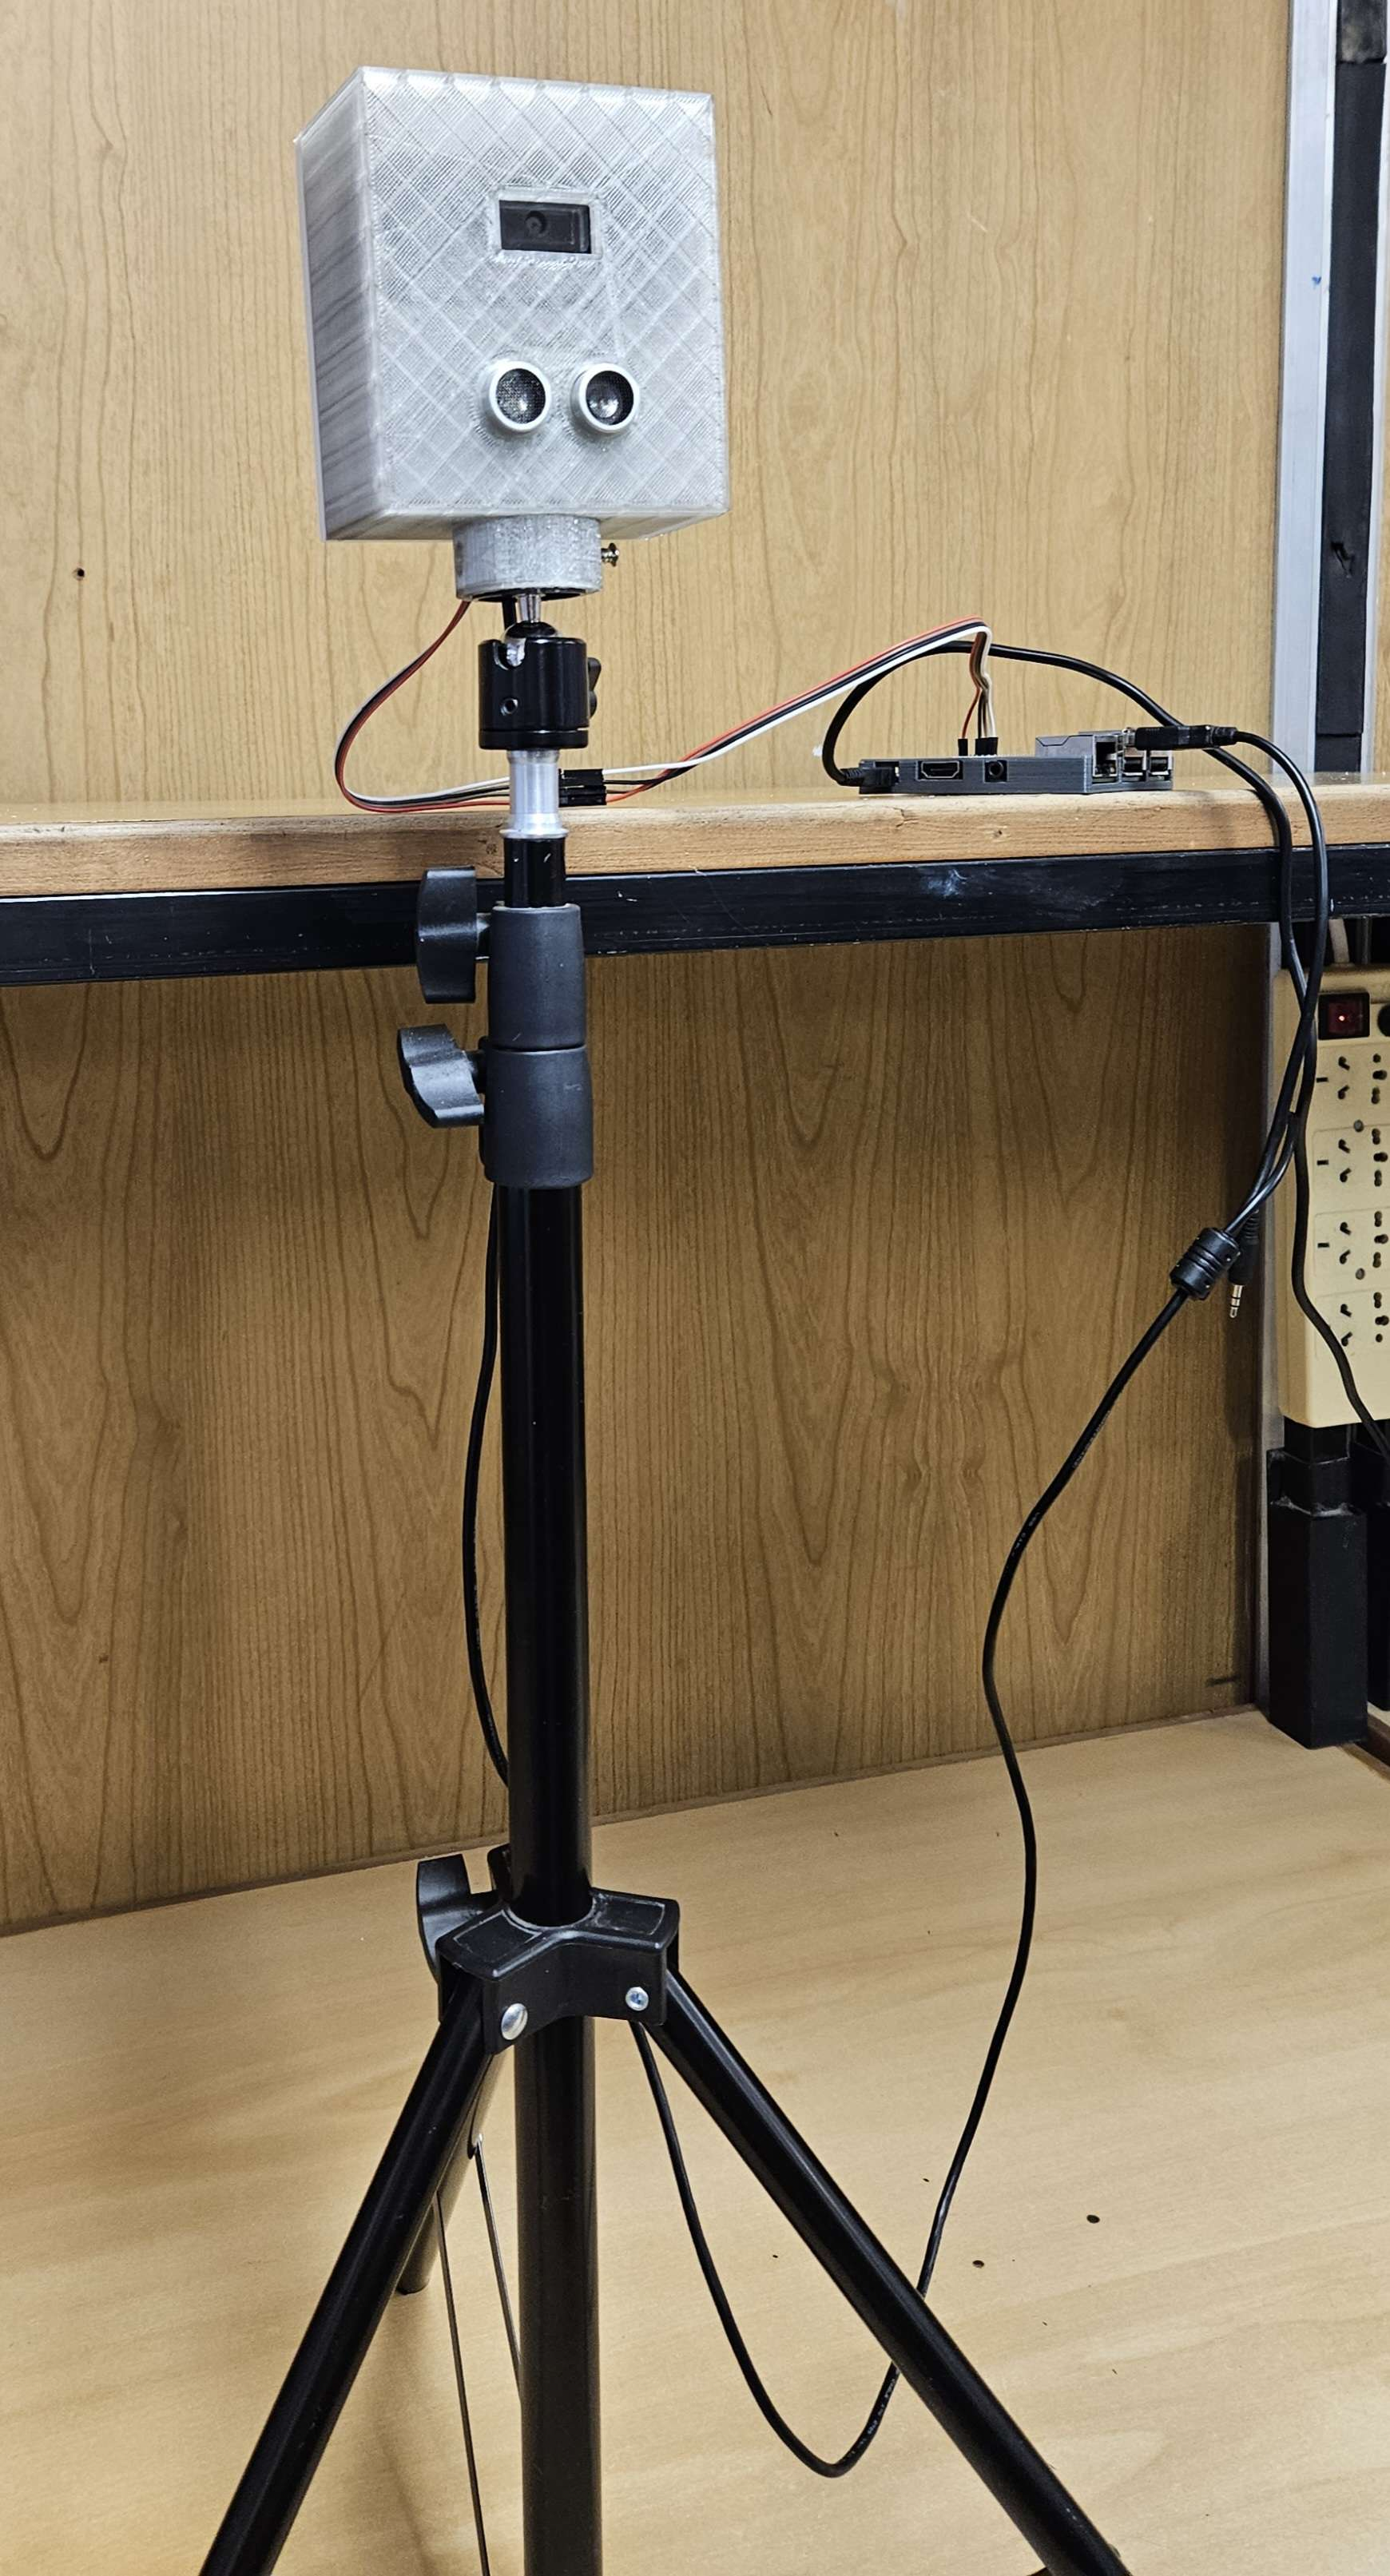
\includegraphics[height=5cm]{imgs/prototipo-sl-mini.jpeg}
        \caption{Protipo SL mini.}
        \label{fig:prot-sl-mini}
    \end{subfigure}
    \caption{Protipos en su estado actual.}
    \label{fig:prototipos}
\end{figure}


